\documentclass[sigconf]{acmart}

\usepackage{graphicx}
\usepackage{hyperref}
\usepackage{todonotes}

\usepackage{endfloat}
\renewcommand{\efloatseparator}{\mbox{}} % no new page between figures

\usepackage{booktabs} % For formal tables

\settopmatter{printacmref=false} % Removes citation information below abstract
\renewcommand\footnotetextcopyrightpermission[1]{} % removes footnote with conference information in first column
\pagestyle{plain} % removes running headers

\newcommand{\TODO}[1]{\todo[inline]{#1}}

\begin{document}
\title{Big Data Analytics for Social Media Threat Intelligence}


\author{Tousif Ahmed}
\orcid{HID237}
\affiliation{%
\institution{Indiana University}
  \streetaddress{150 S Woodlawn Avenue}
  \city{Bloomington} 
  \state{Indiana} 
  \postcode{47405}
}
\email{touahmed@indiana.edu}



\begin{abstract}
Social media has become a virtual society for everyone where billions of people are  interacting  everyday. With the humongous number of users, it has become extremely difficult to manage and track the users behavior in social media.  Malicious actors leverage this weakness of social media platforms and target regular users with threats that includes cyberbullying, malware distribution, spam distribution, fake news, and propaganda.  The consequence of such threats can  affect large number of people, and can result in catastrophic damage. However, identifying the malicious users from the huge number of regular users remain the most challenging problem for the social media platforms. Big data analytics can be one of the most powerful tool  for the social media platforms to prevent the such attacks on social media platforms. This paper discusses the threats of social medias and the ways to use big data analytics to prevent such attacks on social media platforms. 

\end{abstract}

\keywords{E534, HID 237,  Big Data, Social Media, Threat Intelligence, Privacy}


\maketitle



\section{Introduction}
More than two billion people use various social media platforms every day~\cite{social-media}. In every minute, approximately one million people logs in to Facebook, 50,000 photos are uploaded on Instagram, half million tweets are posted on Twitter, two million snaps are created, and one million profile matches happen on Tinder (Figure ~\ref{f:socialmedia}) ~\cite{social-media2}. Social media platforms has become a virtual society for everyone where people are interacting with a large number of audience everyday. Similar to the regular society, there are bad actors in the virtual society who are trying to harm people. Due to the extended outreach, social media platforms has become an ideal platform for the malicious actors to harm that includes cyberbullying ~\cite{Slonje:2013,Kwan:2013,Singh:2017,Cheng:2017,HosseinmardiMRH15} and the distribution of offensive, misleading, false or malicious information ~\cite{Menczer:2016, socialbots-CACM, Shao15hoaxy, Shao17hoaxybots}. Terrorist and government can also leverage social media to spread propaganda~\cite{Aro2016,Weimann:2006}.


\begin{figure}[!ht]
  \centering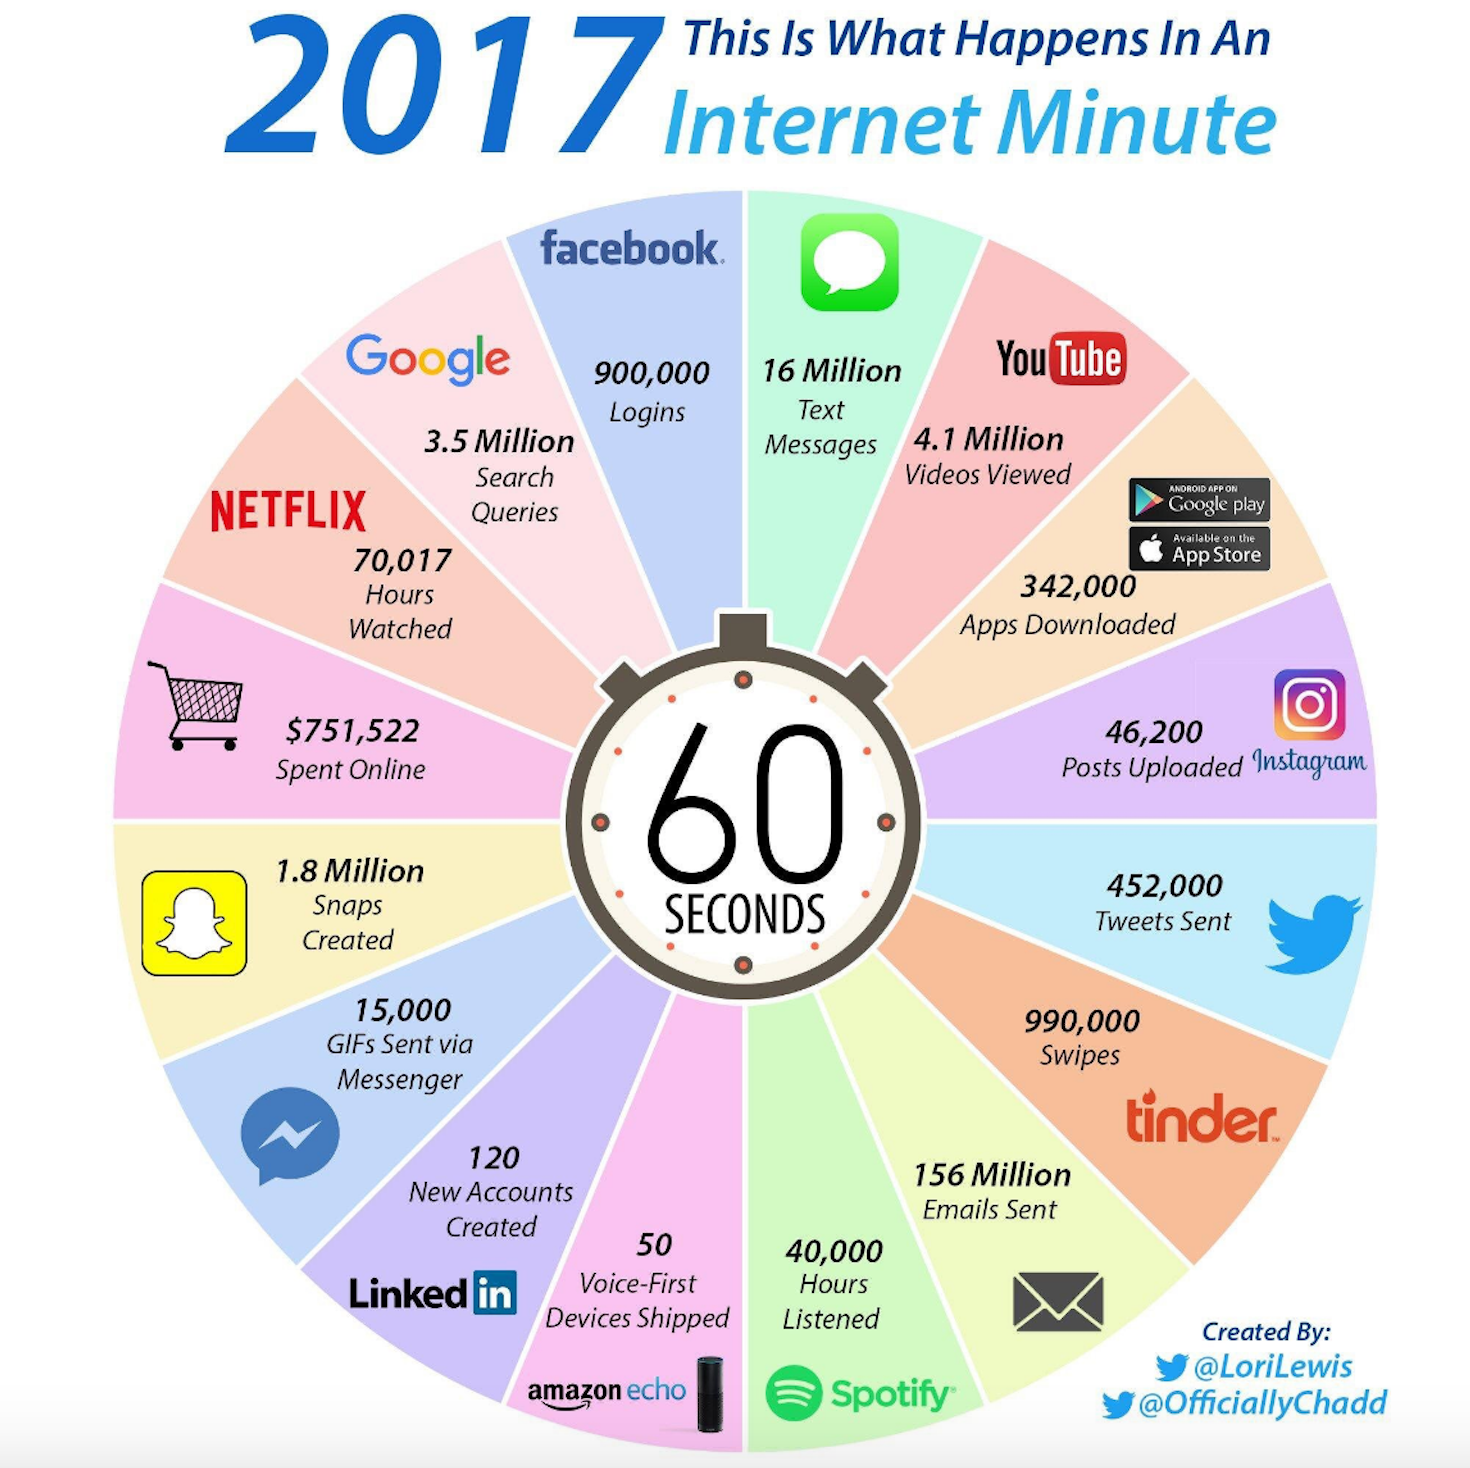
\includegraphics[width=0.5\columnwidth]{images/one-internet-minute.png}
  \caption{What happens in an internet minute?~\cite{social-media2}}\label{f:socialmedia}
\end{figure}

Since the beginning of society, malicious actors are common phenomena and society has taken necessary steps to control them. Law enforcement organizations have been helping the society to control social menaces and protect the individuals from internal and external threats.  Real society constituted by small groups, therefore, it is easier to control  them. In contrast to the actual society, it is far more difficult to manage the virtual society due to it's volume. It is nearly impossible to construct virtual law enforcement organizations in the virtual world and protect the individuals from malicious actors. Therefore, protecting the social media platforms from threats remain one of the most challenging problems. The recent advancement of machine learning and big data shows promises and offer new set of weapons to fight. Big data analytics provides easier way to scale, manage, and visualize user's data which can be valuable for fighting malicious actors. The volume of data gives the researchers tremendous insight which can be a new way to help regular users. This paper discusses the impact of big data on four different social media threats.

\section{Social Media Threat Intelligence}
This section discuss the impact of big data on social media threat intelligence. Each threats were discussed first then the use of big data on detecting and preventing the threats were discussed:

\subsection{Cyberbullying detection and identification}
Cyberbullying can be defined as the usage of computing devices to hurt or embarrass another person.  Cyberbullying in social media constitutes posting negative or offensive comments in posts, post videos or photos to make fun of others,  stalking, harassing, and trolling.  Approximately, 43 percent teenagers in the U.S have been victims of cyberbullying in 2013 and most of them were bullied in social media~\cite{cyberbullying}. Cyberbullying has bad impact on people, which include deep emotional trauma, mental disorder, substance abuse, and suicidal tendency~\cite{cb-effect}. 

The rise of social media has caused significant growth in cyberbullying. The rise of photos and social media have aggravated the situation. However, text analysis or social media post analysis has become impressively smart to detect cyberbullying~\cite{HosseinmardiMRH1}. Natural language processing algorithms like LDA can easily detect social media posts with negative meanings and keyword matching can be helpful to detect and identify the offensive keywords. Recent results shows promising advancement in detecting cyberbullying and in future it would be far easier to control. Another potential approach to detect and identify cyberbullying is analyzing photos or videos.

\subsection{Internal Abuse detection}
Although social media abuse falls in the category of cyberbullying, abuse can be different than cyberbullying. Social media abuse can be defined as misusing user's personal information that do not necessarily harm the user but can break the level of mutual trusts between the abuser and the abused. For example, stealing one's content from their social media profile do not harm the user but breaks the mutual trust in the relationship. In social media, people connect with others by putting a level of trust on others. Sometimes, bad actors can use the information to impersonate the person on social media. Later, the impersonated account can be used to embarrass or demean the victim. This might not be necessary causing mental harm to the victim but misusing the trust. Such bad actors are pretty common in social media. Since the bad actor's are using genuine information, it is very difficult to detect them.

One approach to detect the abusers is to monitor the user's activity. Most of the cases, such actors exhibits some common behavior such as sending friend requests to random people, infrequent usage, random or anomalous behavior and such other behaviors. However, it is not possible for people to monitor the activity of the users to detect the abusers. However, common patterns can be helpful to detect such anomalies and data mining algorithms like k-means can be used to detect such anomalies. Big data analytics can also be helpful to blacklist the social media abusers and additional manual research can be useful to detect the abusers and ban them. 


\subsection{Preventing misinformation}
\subsection{Preventing Terrorism}




\begin{acks}

The authors would like to thank Professor Gregor von Laszewski for helping us with the instruction and resources that was required to complete this paper. We would also to like to thank the associate instructors for being available on the course website all the time and helping us with their answers.

\end{acks}

\bibliographystyle{ACM-Reference-Format}
\bibliography{report} 

\appendix

We include an appendix with common issues that we see when students
submit papers. One particular important issue is not to use the
underscore in bibtex labels. Sharelatex allows this, but the
proceedings script we have does not allow this.

When you submit the paper you need to address each of the items in the
issues.tex file and verify that you have done them. Please do this
only at the end once you have finished writing the paper. To d this
cange TODO with DONE. However if you check something on with DONE, but
we find you actually have not executed it correcty, you will receive
point deductions. Thus it is important to do this correctly and not
just 5 minutes before the deadline. It is better to do a late
submission than doing the check in haste. 

\section{Issues}

\DONE{Example of done item: Once you fix an item, change TODO to DONE}

\subsection{Assignment Submission Issues}

    \TODO{Do not make changes to your paper during grading, when your repository should be frozen.}

\subsection{Uncaught Bibliography Errors}

    \DONE{Missing bibliography file generated by JabRef}
    \DONE{Bibtex labels cannot have any spaces, \_ or \& in it}
    \DONE{Citations in text showing as [?]: this means either your report.bib is not up-to-date or there is a spelling error in the label of the item you want to cite, either in report.bib or in report.tex}

\subsection{Formatting}

    \TODO{Incorrect number of keywords or HID and i523 not included in the keywords}
    \TODO{Other formatting issues}

\subsection{Writing Errors}

    \DONE{Errors in title, e.g. capitalization}
    \DONE{Spelling errors}
    \TODO{Are you using {\em a} and {\em the} properly?}
    \DONE{Do not use phrases such as {\em shown in the Figure below}. Instead, use {\em as shown in Figure 3}, when referring to the 3rd figure}
    \DONE{Do not use the word {\em I} instead use {\em we} even if you are the sole author}
    \TODO{Do not use the phrase {\em In this paper/report we show} instead use {\em We show}. It is not important if this is a paper or a report and does not need to be mentioned}
    \DONE{If you want to say {\em and} do not use {\em \&} but use the word {\em and}}
    \DONE{Use a space after . , : }
    \DONE{When using a section command, the section title is not written in all-caps as format does this for you}\begin{verbatim}\section{Introduction} and NOT \section{INTRODUCTION} \end{verbatim}

\subsection{Citation Issues and Plagiarism}

    \DONE{It is your responsibility to make sure no plagiarism occurs. The instructions and resources were given in the class}
    \DONE{Claims made without citations provided}
    \DONE{Need to paraphrase long quotations (whole sentences or longer)}
    \DONE{Need to quote directly cited material}

\subsection{Character Errors}

    \DONE{Erroneous use of quotation marks, i.e. use ``quotes'' , instead of " "}
    \DONE{To emphasize a word, use {\em emphasize} and not ``quote''}
    \DONE{When using the characters \& \# \% \_  put a backslash before them so that they show up correctly}
    \DONE{Pasting and copying from the Web often results in non-ASCII characters to be used in your text, please remove them and replace accordingly. This is the case for quotes, dashes and all the other special characters.}
    \DONE{If you see a figure and not a figure in text you copied from a text that has the fi combined as a single character}

\subsection{Structural Issues}

    \DONE{Acknowledgement section missing}
    \DONE{Incorrect README file}
    \DONE{In case of a class and if you do a multi-author paper, you need to add an appendix describing who did what in the paper}
    \TODO{The paper has less than 2 pages of text, i.e. excluding images, tables and figures}
    \TODO{The paper has more than 6 pages of text, i.e. excluding images, tables and figures}
    \TODO{Do not artificially inflate your paper if you are below the page limit}

\subsection{Details about the Figures and Tables}

    \DONE{Capitalization errors in referring to captions, e.g. Figure 1, Table 2}
    \DONE{Do use {\em label} and {\em ref} to automatically create figure numbers}
    \DONE{Wrong placement of figure caption. They should be on the bottom of the figure}
    \DONE{Wrong placement of table caption. They should be on the top of the table}
    \DONE{Images submitted incorrectly. They should be in native format, e.g. .graffle, .pptx, .png, .jpg}
    \DONE{Do not submit eps images. Instead, convert them to PDF}

    \DONE{The image files must be in a single directory named "images"}
    \DONE{In case there is a powerpoint in the submission, the image must be exported as PDF}
    \DONE{Make the figures large enough so we can read the details. If needed make the figure over two columns}
    \DONE{Do not worry about the figure placement if they are at a different location than you think. Figures are allowed to float. For this class, you should place all figures at the end of the report.}
    \DONE{In case you copied a figure from another paper you need to ask for copyright permission. In case of a class paper, you must include a reference to the original in the caption}
    \DONE{Remove any figure that is not referred to explicitly in the text (As shown in Figure ..)}
    \DONE{Do not use textwidth as a parameter for includegraphics}
    \DONE{Figures should be reasonably sized and often you just need to
  add columnwidth} e.g. \begin{verbatim}/includegraphics[width=\columnwidth]{images/myimage.pdf}\end{verbatim}



\end{document}
